%----------------------------------------------------------------------------------------
%    PACKAGES AND THEMES
%----------------------------------------------------------------------------------------

\documentclass[aspectratio=169,xcolor=dvipsnames]{beamer}
\usetheme{SimplePlus}

\usepackage{hyperref}
\usepackage{graphicx} % Allows including images
\usepackage{booktabs} % Allows the use of \toprule, \midrule and \bottomrule in tables

%----------------------------------------------------------------------------------------
%    TITLE PAGE
%----------------------------------------------------------------------------------------

\title{Lazy Search Trees}
\subtitle{Introduction}

\author{Rafał Włodarczyk}

\institute
{
    INA 4
}
\date{\today} % Date, can be changed to a custom date

%----------------------------------------------------------------------------------------
%    PRESENTATION SLIDES
%----------------------------------------------------------------------------------------

\begin{document}

\begin{frame}
    \titlepage
\end{frame}

\begin{frame}{Overview}
    \tableofcontents
\end{frame}

%------------------------------------------------

\section{Introduction}
\begin{frame}{A Brief History of Tree Data Structures}
    These tree data structures had the biggest impact on the field:
    \begin{itemize}
        \item \textbf{Binary Search Tree (1960s)} $O(\log n)$ average-case query, $O(n)$ worst-case query.
        \item \textbf{AVL Tree (1962)} Self-balancing, $O(\log n)$ worst-case for insert and query.
        \item \textbf{Red-Black Tree (1972)} Self-balancing, $O(\log n)$ worst-case for insert and query, often with fewer rotations than AVL.
        \item \textbf{Splay Tree (1985)} Self-adjusting, performance optimized for sequences of operations. Frequently queried keys are closer to the root node.
        \item \textbf{Treap (1989)} Randomized, combines properties of binary search trees and heaps.
    \end{itemize}
    Building on research into Deferred Tree Structures, the \textbf{Lazy Search Tree (2020)} introduces postponed updates and efficiency for specific query patterns.
\end{frame}

%------------------------------------------------

\section{Problem Domain}
\begin{frame}{Problem Domain}
    Assume the comparison model and consider a dynamic multiset $S$ of (current) size $|S|=n$. Our goal is to efficiently support two types of operations:

    \begin{itemize}
        \item order-based operations: rank, select, membership, predecessor, successor, minimum, and maximum.
        \item dynamic operations: insert, delete, change-key, split, and merge.
    \end{itemize}

    \vspace{0.5cm}

    Example: if we only want to support minimum and maximum element we are left with a \textbf{priority queue}. 
    We therefore aim for a generalization of priority queues, which provide all of the order-based operations from above.

    \vspace{0.25cm}

    Performance-wise, we want to get as close to a dictionary implemented with a hash table, while supporting the order-based operations
    - ultimately achieving what is known as a \textbf{sorted dictionary}.
\end{frame}

%------------------------------------------------

\section{Sorted Dictionary Interface}
\begin{frame}{Sorted Dictionary Interface}
    The paper proposes the following interface to define a sorted dictionary:

    \begin{itemize}
        \item \textbf{Construction(S)} Construct a sorted dictionary on the set $S$.
        \item \textbf{Insert(e)} Add $(k, v)$ to $S$, where $k$ is a comparable key.
        \item \textbf{RankBasedQuery(r)} A general rank-based query on $S$. Example. $r$-th smallest element.
        \item \textbf{Delete(ptr)} Delete the element pointed to by \texttt{ptr} from $S$.
        \item \textbf{ChangeKey(ptr, k')} Change the key of the element pointed to by \texttt{ptr} to $k'$.
        \item \textbf{Split(r)} Split $S$ at rank $r$, returning two sorted dictionaries $T_1$ and $T_2$ of $r$ and $n - r$ elements, respectively, which satisfy $\left(\forall x \in T_1\right)\left(\forall y \in T_2\right)\left(x \leq y\right)$.
        \item \textbf{Merge(T$_1$, T$_2$)} Merge sorted dictionaries $T_1$ and $T_2$ and return the result, which satisfies $\left(\forall x \in T_1\right)\left(y \in T_2\right)\left(x \leq y\right)$.
    \end{itemize}

\end{frame}

%------------------------------------------------

\section{Gaps}
\begin{frame}{Gaps}
    We maintain a set of $m$ gaps $\{\Delta_i\}$, $1 \leq i \leq m$, where each gap $\Delta_i$ contains a bag of elements. 
    The gaps satisfy \textbf{the total order property} - $\left(\forall x \in \Delta_i\right)\left(y \in \Delta_{i+1}\right)\left(x \leq y\right)$.

    \vspace{0.25cm}

    Example 1. Take an example multiset $S = \{(1,a),(1,a),(3,c),(4,d)\}$, composed of pairs $(k_i,v_i)$, we can represent it as a set of gaps, which satisfy the total order on $k_i$.
    \begin{align*}
        \Delta_1 = \{(1,a)\} \quad \Delta_2 = \{(1,a)\} \quad \Delta_3 = \{(3,c)\} \quad \Delta_4 = \{(4,d)\}
    \end{align*}

    Example 2. We could also define it as:
    \begin{align*}
        \Delta_1 = \{(1,a),(1,a)\} \quad \Delta_2 = \{(3,c),(4,d)\}
    \end{align*}
\end{frame}

%------------------------------------------------

\begin{frame}{Gap insertion and deletion}
    Example 3. Let's insert a new element $(k,v)=(3,b)$ to gaps from Example 1. We must maintain the total order property,
    therefore we find a gap, such that:
    \begin{align*}
        \left(\forall k_i\in\Delta_i\right)\left( \forall k_{i+1}\in\Delta_{i+1}\right) k_i \leq k < k_{i+1}
    \end{align*}
    
    Which in this case is $\Delta_2$ or $\Delta_3$. We insert the element into the gap, resulting in:

    \begin{align*}
           \Delta_1 = \{(1,a)\} \quad \Delta_2 = \{(1,a)\} \quad \Delta_3 = \{(3,c), (3,b)\} \quad \Delta_4 = \{(4,d)\}
    \end{align*}

    Alternatively:

    \begin{align*}
           \Delta_1 = \{(1,a)\} \quad \Delta_2 = \{(1,a), (3,b)\} \quad \Delta_3 = \{(3,c)\} \quad \Delta_4 = \{(4,d)\}
    \end{align*}

    The paper specifies both are valid, and the choice is left to the implementation.
    
    \vspace{0.1cm}

    Deletion happens similarly, we find the gap containing the element to be deleted, and remove it from the bag - if the bag is empty, we remove the gap itself.
\end{frame}

%------------------------------------------------

\section{Intervals}
\begin{frame}{Intervals}
    Within each gap $\Delta_i$, elements are further partitioned into intervals. Each interval is defined by a pair of keys $(k_l, k_r)$. The interval only contains a key $k$ if $k_l \leq k \leq k_r$.

    Example. For the gap $\Delta_t$:

    \begin{align*}
        \Delta_t = \{(1,a), (1,b), (2,c), (3,d)\}
    \end{align*}

    We can present the following interval representation:

    \begin{align*}
        \mathcal{I} = \{(1,2), (3,3)\}
    \end{align*}

    The paper proves there are at most $4\log(|\Delta_i|)$ intervals in each $\Delta_i$ gap.
\end{frame}

%------------------------------------------------

\section{LST - Lazy Search Tree}
\begin{frame}{Lazy Search Tree}

The data structure has two levels:

\begin{itemize}
    \item \textbf{The Gaps} $\{\Delta_i\}$ at the top level. Within each \textbf{gap} $\{\Delta_i\}$, there are:
    \item \textbf{The Intervals} $\mathcal{I}_{i,1},\mathcal{I}_{i,2},\dots,\mathcal{I}_{i,\ell_i}$, where $\ell_i$ is \# of intervals in gap $\Delta_i$.
\end{itemize}

\begin{figure}[h]
    \centering
    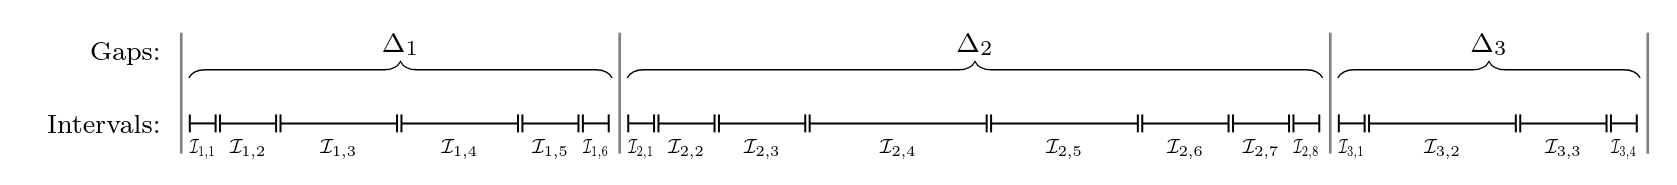
\includegraphics[width=0.8\linewidth]{lst.png}
    \caption{Visualization of a Lazy Search Tree.}
\end{figure}

We can store the gaps using a globally biased $(2,B)$-Tree and the intervals as a sorted array.

\end{frame}

%------------------------------------------------

\begin{frame}{LST - Construction}
Let us insert the sequence: $5, 12, 3, 8, 15, 6$.

\begin{itemize}
    \item \textbf{Initial} $\{\}$.
    \item \textbf{Add 5} $\Delta_1 = \{5\}$
    \item \textbf{Add 12} $\Delta_1 = \{5, 12\}$
    \item \textbf{Add 3} $\Delta_1 = \{3\}, \Delta_2 = \{5, 12\}$
    \item \textbf{Add 8} $\Delta_1 = \{3\}, \Delta_2 = \{5, 8, 12\}$
    \item \textbf{Add 15} $\Delta_1 = \{3\}, \Delta_2 = \{5, 8, 12, 15\}$
    \item \textbf{Add 6} $\Delta_1 = \{3\}, \Delta_2 = \{5, 6, 8, 12, 15\}$
\end{itemize}

\vspace{1cm}

Construction inevitably runs in $O(n)$ time.

\end{frame}

%------------------------------------------------

\section{LST - Insertion}
\begin{frame}[fragile]{LST - Insertion}

We either create a new gap $\Delta_1$ or find the smallest $i$, such that $\left(\forall k\in\Delta_i\right) \left(\text{key} \geq k\right)$

\begin{verbatim}
void insert(const T &key) {
    if (empty()) {
        gap r_gap = gap(key);
        gap_ds.insert(r_gap);
    } else {
        gap& r_gap = gap_ds.lower_bound_or_last(gap(key));
        r_gap.insert(key);
    }
    ++lst_size;
}
\end{verbatim}

Lower bound or last gap - $\Delta_i$ can be found with binary search in $O\left( \log\frac{n}{\Delta_i} \right) $. There are at most $O\left( \log \Delta_i \right)$ intervals in $\Delta_i$. Binary search to find an interval then runs in $O\left( \log \log \Delta_i \right)$ time. Therefore the whole insert runs in $O\left(\log\frac{n}{\Delta_i} + \log \log \Delta_i \right)$.
\end{frame}

%------------------------------------------------

\begin{frame}{LST - Insertion Example with Intervals}
Assume LST: $\Delta_1 = \{3\}, \Delta_2 = \{5, 6, 8, 12, 15\}$, with intervals
$\mathcal{I}_{1,1}=[3,3],\mathcal{I}_{2,1}=[5,6,8],\mathcal{I}_{2,2}=[12,15]$ and we want to insert $\text{key}=9$.

\begin{enumerate}
    \item Find the relevant gap. The \texttt{lower\_bound\_or\_last} function selects $\Delta_2$ as the first target gap, since $9 > 3$.
    \item Find the interval within gap. Within $\Delta_2$, $9$ falls between the elements of $\mathcal{I}_{2,1}$ and $\mathcal{I}_{2,2}$.
    \item Place $9$ in $\Delta_2$ in its sorted position. Update gaps or intervals depending on the situation - must maintain the total order property and not degenerate the structure.
\end{enumerate}

We end up with LST: $\Delta_1 = \{3\}, \Delta_2 = \{5, 6, 8, 9, 12, 15\}$, with intervals $\mathcal{I}_{1,1}=[3,3], \mathcal{I}_{2,1}=[5,6,8]$, $\mathcal{I}_{2,2}=[9,9]$, $\mathcal{I}_{2,3}=[12,15]$).

\end{frame}

%------------------------------------------------

\begin{frame}[fragile]{How intervals are found in code}
\begin{verbatim}
int getIntervalIdx(const T &key) {
  int lo = last_left_idx, hi, mult;
  bool init = key <= intervals[last_left_idx]->get_max();
  mult = (init) ? -1 : 1;

  exponential_search(lo, hi, mult, init, key, intervals);
  return binary_search(lo, hi, init, key, intervals);
}
\end{verbatim}

Paper states it is optimized to provide $O(1)$ average case insert, $O(\log\log \Delta_i)$ worst case.
\end{frame}

%------------------------------------------------

\section{LST - Query}
\begin{frame}{LST - Query}
    When performing a query, we first identify the gap $\Delta_i$ that contains the rank element $r$. Formally, we find $i$ such that:
    \[
    \sum_{j=1}^{i-1} |\Delta_j| < r \leq \sum_{j=1}^{i} |\Delta_j|.
    \]
    We then answer the query using the elements within $\Delta_i$.

    During this process, we can restructure the gaps by splitting $\Delta_i$ into two new gaps, $\Delta'_i$ and $\Delta'_{i+1}$, keeping the total order property. The split is performed so that the rank element $r$ is the largest in $\Delta'_i$ or the smallest in $\Delta'_{i+1}$. Specifically, after the split, either
    \[
    |\Delta'_i| + \sum_{j=1}^{i-1} |\Delta_j| = r \quad \text{or} \quad  |\Delta'_i| + \sum_{j=1}^{i-1} |\Delta_j| = r - 1.
    \]
    This ensures that the structure remains consistent and supports efficient future queries.
\end{frame}

%------------------------------------------------

\section{LST - Update on Query}
\begin{frame}{LST - Update on Query}

After each query we can perform an update.

\begin{figure}[h]
    \centering
    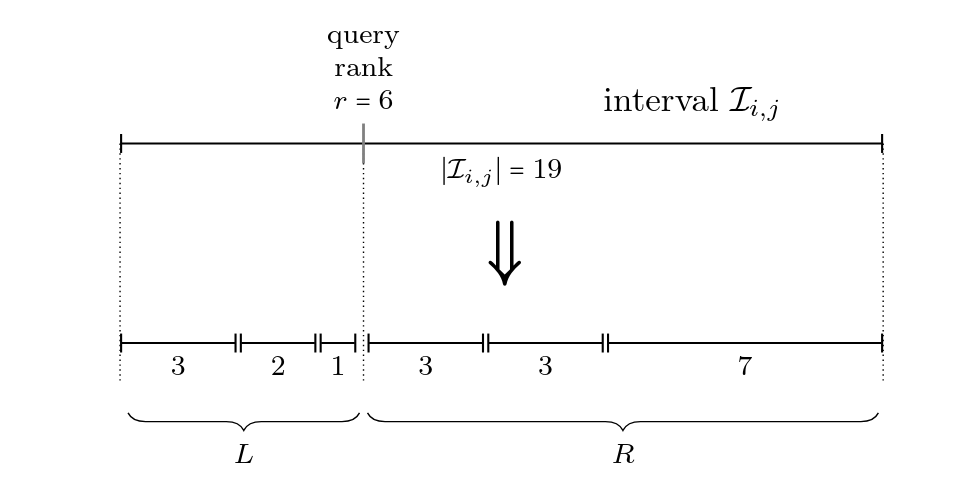
\includegraphics[width=0.8\linewidth]{lst2.png}
    \caption{Visualization of an interval update.}
\end{figure}

\end{frame}

\section{LST - Count function}
\begin{frame}[fragile]{LST - Count function}

\begin{verbatim}
bool membership(const T &key) {
  return intervals[getIntervalIdx(key)]->membership(key);
}

int count(const T &key) {
    if (empty()) return false;
    gap &r_gap = gap_ds.lower_bound_or_last(gap(key));
    bool result = r_gap.membership(key);
    
    pair<gap, gap> new_gaps = r_gap.restructure(key, 2);
    gap_ds.erase(r_gap); 
    if (!new_gaps.first.empty())  gap_ds.insert(new_gaps.first);
    if (!new_gaps.second.empty()) gap_ds.insert(new_gaps.second);
    return result;
}
\end{verbatim}

\end{frame}


%------------------------------------------------

\begin{frame}{LST - Chained Queries}
The Lazy Search Tree adapts its efficiency based on query distribution.

\begin{itemize}
    \item \textbf{General Case}. Over a sequence of $n$ insertions and $q$ distinct queries, the total complexity is $O(B + \min(n \log \log n, n \log q))$. $B = \Sigma_{i=1}^{m} |\Delta_i| \log_2(n/|\Delta_i|)$ is defined in the abstract. A time bound of $O(n \log q + q \log n)$ holds.
    \item \textbf{Few Queries}. If $q$ is small (e.g., $q=O(1)$), lazy search trees can achieve near-linear time for the sequence.
    \item \textbf{Clustered Queries}. For $q/k$ queries each requesting $k$ consecutive keys, with uniform insertions in between, the total cost is $O(n \log(q/k) + \min(n \log \log n, n \log q))$ for insertions and $O(\log n)$ for successive queries within a batch after the first query.
    \item \textbf{Priority Queue}. If all queries are for the minimum element, the Lazy Search Tree functions as a priority queue. Insertions take $O(\log \log n)$ time, and each query takes $O(\log n)$ time.
\end{itemize}
\end{frame}

%------------------------------------------------

\section{References}
\begin{frame}{References}
    \begin{enumerate}
        \item Sandlund, Bryce, and Sebastian Wild. "Lazy search trees." 2020 IEEE 61st Annual Symposium on Foundations of Computer Science (FOCS). IEEE, 2020. \url{https://arxiv.org/abs/2010.08840}
        \item Sandlund, Bryce. "Lazy Search Trees (GitHub repository)." \url{https://github.com/brycesandlund/lazy-search-trees}
    \end{enumerate}
    Further read: 
    \begin{enumerate}
        \item Rysgaard, Casper Moldrup, and Sebastian Wild. "Lazy B-Trees." arXiv preprint arXiv:2507.00277 (2025). \url{https://arxiv.org/abs/2507.00277}
    \end{enumerate}
\end{frame}

%----------------------------------------------------------------------------------------

\end{document}